\section{背\ 景}\label{sec:background}

\subsection{微服务(MicroService)}
微服务(Microservice)~\cite{lewis2014microservices}是一种基于服务架构(Service-Oriented Architecture,SOA)~\cite{papazoglou2007service}的软件设计风格和架构模式,将单一应用(Monolithic)程序拆分为一组独立的、小型的微服务,每个微服务都可以独立开发、部署、扩展、升级,已被广泛应用于云计算、容器化、DevOps等领域,是现代软件开发中的重要架构之一。

相比于传统的单一服务模式,微服务主要具备以下的优势:

\begin{itemize}
    \item \textbf{模块化}:微服务节点间是松耦合的,各微服务可以独立开发、部署和升级,模块化程度很高。
    \item \textbf{隔离性}:每个微服务都是独立自治的系统,一个微服务的故障不会影响其他微服务的运行,更不会导致整个系统的崩溃,可以很好的实现故障隔离,从而提高了系统的可用性。
    \item \textbf{可扩展性}:庞大的单一应用如果出现性能瓶颈,只能对整个应用进行扩容,但是真正的瓶颈可能只是其中一个模块,整体扩展会带来大量的资源浪费;而微服务可以根据实际情况只对限制性能的微服务进行弹性扩容,从而提高了系统的可扩展性。
    \item \textbf{异构性}:由于微服务节点间独立、网络通信的特点,只要需要通信的节点间协定好通信协议,不同节点可以采用异构的开发语言、框架、硬件架构等,从而可以根据业务需求选择最适合的技术栈,提高了开发的灵活性。
    \item \textbf{简化部署}:传统单一应用的升级部署需要对整个应用重新打包并重新部署,这样非常复杂且充满不确定性;而微服务架构可以对每个微服务进行独立的升级部署,不需要影响其他节点,从而提高了升级部署的效率。
\end{itemize}

但是作为一种分布式的架构,微服务无疑也带来了许多新的挑战,包括服务安全、服务间通信、服务鉴权与认证、服务注册与发现、服务负载均衡、服务容器化等。本次研究主要聚焦于安全计算的微服务场景,需要着重考虑并解决服务的安全性、可信度和通信方面的问题。

\subsection{平台即服务(PaaS)}

平台即服务(Platform-as-a-Service,简称PaaS)~\cite{mell2011nist}是云计算场景的一种服务模式,提供了应用程序开发和部署所需的平台和工具,开发者可以使用这些来开发、测试和部署自己的应用程序,而无需考虑底层的基础设施和资源管理等问题。PaaS通常提供了操作系统、开发环境、数据库管理系统、Web服务器等平台和工具,这些都运行在公有云的基础设施上,无需开发者进行维护,使得开发者可以更加专注于应用程序的开发和业务逻辑。PaaS提供的资源可以根据应用需要进行弹性分配和弹性扩容,从而提高了应用程序的可扩展性。

得益于PaaS的便利性,越来越多的企业和开发者选择将自己的微服务应用部署到PaaS平台上,以降低应用开发和部署的成本。但是PaaS作为一种公有云提供服务的方式,部署在其上的应用需要信任PaaS平台的安全性,而传统情况下这一点无法得到保障:一个恶意的或被恶意攻击者劫持的PaaS平台可以在更高的特权级下轻松获取应用的隐私数据。这一点大大限制了PaaS的使用场景,导致涉及隐私数据的公有云使用遭到了严重挑战。

\subsection{可信执行环境(TEE)}

可信执行环境是一种结合硬件和密码学原理的可信计算技术,通过在不可信的环境中创建一个可信的、隔离的飞地(Enclave),使用特殊的硬件指令控制加密数据进出飞地并在其中解密进行计算,达到高特权级的操作系统(OS)或Hypervisor也无法获取机密数据的能力,从而保护应用程序的安全性。在分布式场景下,TEE通过结合硬件的方式,可以达到与安全多方计算(MPC)~\cite{afram2014theory}、同态加密(HE)~\cite{gentry2009fully}相似的安全保障,但是由于MPC和HE需要复杂的计算和使用逻辑,效率远远不如TEE。然而,TEE的硬件可能会受到侧信道攻击~\cite{oleksenko2018varys}、时序攻击等物理攻击,从而导致TEE的安全性受到威胁;目前针对这些攻击已有一定的研究和防御手段~\cite{oleksenko2018varys}。

可信执行环境的实现包括Intel的SGX~\cite{costan2016intel}、ARM的TrustZone~\cite{arm2009security}、AMD的SEV~\cite{kaplan2016amd}以及RISC-V上开源的Keystone~\cite{lee2020keystone}等。由于目前主流的PaaS底层硬件多是Intel架构的,因此我们对于TEE的使用主要聚焦于Intel SGX。SGX(Software Guard Extensions)~\cite{costan2016intel}实现了基于机器安全内存检查机制支持的一组指令集扩展,设计了内存保护和地址映射保护规则,并设计了远程验证协议,由此可以为受保护的内存提供机密性和完整性保障,而不依赖于软件和固件的实现,可以轻松抵御特权态攻击。

\subsection{库操作系统(Library OS)}

库操作系统(Library Operating System,简称LibOS)~\cite{engler1995exokernel}是一种将操作系统内核提供的资源管理、系统调用等功能以库的形式提供给应用程序的操作系统,具有模块化、专用化、单地址空间的特点。相比于传统的操作系统,由于功能在库中实现,开发者可以根据自己的需要对库进行定制和扩展,从而使LibOS可以更加轻量级、更加灵活地提供需要的功能,从而提高应用程序的性能和可扩展性。

因为SGX本质上是硬件隔离的内存区域,上面只有很少的库函数,不能提供POSIX接口功能,因此想要将外部程序放到SGX中运行,可以使用LibOS提供运行时环境,达到不需要更改或极少更改源程序的目的。可以在SGX中运行的LibOS有Graphene-SGX~\cite{tsai2017graphene}、Occlum~\cite{shen2020occlum}等。

\subsection{远程验证协议}

远程验证协议是一种用于验证远程实体的安全性和完整性的协议。通常会在一个可信的环境中运行,用来确保远程设备的代码和数据没有被篡改或者受到攻击。

SGX远程验证(SGX remote attestation)~\cite{intel-sgx-ra}是Intel SGX提供的一种远程验证协议,用于证明远程节点身份可信、内容未被篡改、运行在合法的SGX实体中、安全级别正确,由此可以确保被验证的程序是预期的版本、未被篡改、是由一个受信任的源发布的、并且安全地运行在SGX上。

为了进行远程验证,Intel提供的SGX SDK提供了创建QUOTE的结构,QUOTE中保存了飞地的身份和运行平台的信息;Intel还提供了Intel Attestation Service(IAS),这是一种可以使用组签名方案验证QUOTE真实性的服务~\cite{intel-sgx-ra}。另外,Intel SGX建立了2个识别飞地的度量标准(measurement),分别是飞地身份(the enclave identity)和密封身份(the sealing identity)。飞地身份即MRENCLAVE,是一个SHA-256摘要,取自飞地构建过程中所有活动(包括飞地中页面的相对位置、页面的安全标志及页面内容等)的日志;而密封身份包括密封授权机构、产品ID和版本号,密封授权机构通常是飞地的构建者,其签署了一个RSA飞地证书(SIGSTRUCT),其中包含MRENCLAVE和验证签名的公钥,验证通过后计算密封授权机构公钥的哈希值,即为MRSIGNER。

在远程验证过程中涉及三个参与方:挑战者(Challenger)、被验者(Attester)和IAS。挑战者是发起验证的一方,被验者是被验证的一方,IAS是被验者和挑战者之间的信任第三方。

\begin{figure}[!ht]
    \centering
    \includegraphics[width=.7\textwidth]{figures/sgx-ra.png}
    \caption{SGX官网的远程验证完整流程图}
    \label{fig:sgx-ra}
\end{figure}

图\ref{fig:sgx-ra}描述了SGX远程验证的过程,其中描绘的消息流简述如下:

\begin{itemize}
    \item \textbf{消息 0}:挑战者将其公钥发送给被验者,表示开始新的认证过程。
    \item \textbf{消息 1}:被验者收到消息0后,使用该公钥创建DHKE~\cite{diffie2022new}的上下文,并将自己的公钥发送给挑战者。% TODO:引用参考uranus这里的引用
    \item \textbf{消息 2}:挑战者使用DHKE算法导出对称共享密钥(SK),并生成消息2,其中包含挑战者的公钥、两个公钥(挑战者和被验者)的串联签名以及使用共享密钥生成的消息验证码(MAC)。
    \item \textbf{消息 3}:被验者检查消息2并借助Quoting Enclave(QE)创建QUOTO,并用SK生成MAC,包含在消息3中。
    \item \textbf{QUOTE检查}:挑战者验证MAC并将QUOTE发送给IAS。IAS验证QUOTE的签名和结构,然后用认证验证报告(AVR)回答。如果AVR状态为“OK”,则挑战者可以信任QUOTE的内容,并将其与参考值(期望的MRENCLAVE或MRSIGNER)进行比较。
    \item \textbf{消息 4}:挑战者确认远程验证通过,之后挑战者可以将机密信息发送给被验者。
\end{itemize}

\subsection{传输层安全协议(TLS)}

传输层安全协议(Transport Layer Security,简称TLS)~\cite{8446},其前身为安全套接层(Secure Sockets Layer,简称SSL),是一种基于加密技术的安全协议,目的是为互联网通信提供机密性、完整性保障。TLS可以用来防御中间人攻击(MITM)、重放攻击(Replay Attack)等~\cite{8446},可以无耦合的为高层应用协议(例如HTTP)提供安全支持,因此广泛应用于网络通信中。

TLS协议在传输层协议(例如TCP)建立连接后,首先通过握手协议交换信息协商对称密钥,建立安全连接,然后加密数据传输。目前最新的TLS版本为TLS 1.3~\cite{8446},在之前版本的基础上放弃了安全性较低的加密算法,优化了握手协议使其能够1-RTT完成(如图\ref{fig:1-rtt}所示),并初步支持了0-RTT状态恢复机制。但是TLS的0-RTT恢复方式可能会引起重放攻击,目前已有的研究(例如Anti-Replay~\cite{8446}等)可能会引起额外的计算和资源消耗。

\begin{figure}[!ht]
    \centering
    
\includegraphics[width=.7\textwidth]{figures/1-RTT.svg}
    \caption{TLS 1.3初始1-RTT握手流程}
    \label{fig:1-rtt}
\end{figure}

\subsection{Diffie-Hellman密钥交换(DHKE)算法}

Diffie-Hellman密钥交换(DHKE)算法~\cite{diffie2022new}是SGX远程验证协议和TLS握手协议使用的一种重要生成对称密钥的算法。该算法的基本思想是,两个通信方通过交换各自的部分公开信息,结合自己的私有信息计算出一个共享的对称密钥。DH算法基于离散对数问题,其安全性依赖于离散对数问题的难解性,即给定素数p、整数g和$g^x$,求x的值。DH算法的具体过程如图\ref{fig:dhke}所示:

\begin{figure}[!ht]
    \centering
    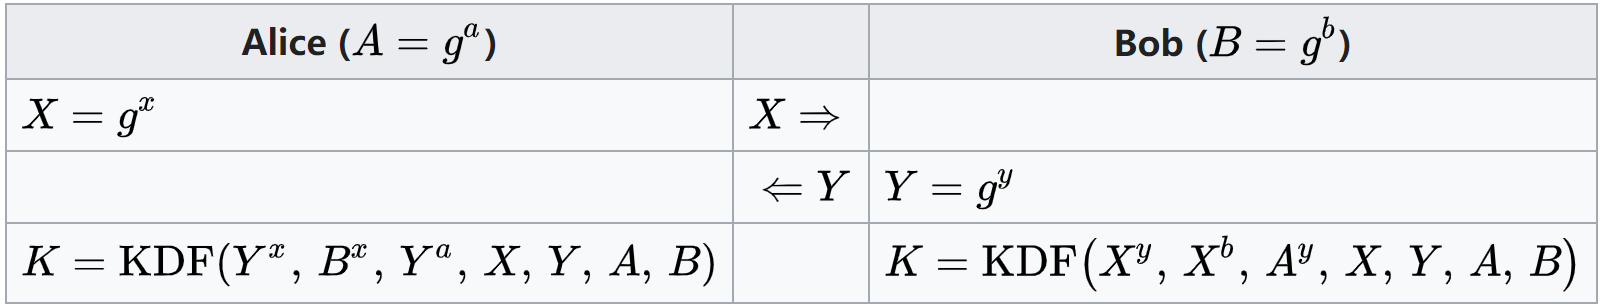
\includegraphics[width=.7\textwidth]{figures/DHKE.svg}
    \caption{DHKE算法示意图}
    \label{fig:dhke}
\end{figure}


\begin{enumerate}
    \item 通信双方Alice和Bob首先公开素数p和整数g,g为p的原根。
    \item Alice选择随机数a,并将$g^a mod p$发送给Bob。
    \item Bob选择随机数b,并将$g^b mod p$发送给Alice。
    \item Alice和Bob分别计算$(g^b mod p)^a mod p$和$(g^a mod p)^b mod p$,得到的结果相同,即为对称密钥。
\end{enumerate}

在此过程中,恶意攻击者Eve即使截获了所有信息,也无法计算出对称密钥,因为她无法解决离散对数问题。

% TODO:思考,这个真的有必要作为背景出现吗?
\subsection{令牌(Token)授权}\label{subsec:token}

令牌(Token)是一种用于身份验证和授权的加密字符串。在SOA架构中,Token是一种常见的认证和授权机制,例如传统单一应用中客户端(Client)可以向服务端(Server)传递Token证明自己的身份信息和拥有的权限。但在微服务场景中,除了Client向API网关传递Token进行认证和授权,在微服务节点间也需要携带Token,否则可能会导致未经授权的节点访问到机密信息,造成隐私泄露。同时为了减小隐私扩散,需要设计细粒度的Token认证和授权模式。JWT(JSON Web Token)~\cite{rfc7519}是一种常见的Token格式,具有自包含、可扩展、跨语言的特点,符合微服务细粒度、异构性的要求,已得到广泛应用。

目前微服务中基于JWT的验证结构中,API网关和Client之间的验证类似于传统单一应用Server和Client之间的验证,而微服务节点间的设计思路有以下4种方式:

\begin{itemize}
    \item API网关通过验证后,将不改变的JWT传递给下级微服务节点,下级微服务节点再次验证Token。这种方式需要多次验证、不够灵活,且JWT中包含的额外权限信息可能会泄露给下级微服务节点。
    \item API网关通过后,后续不再传递JWT,服务节点默认信任API网关的验证结果。这种方式避免了重复验证的开销,但是可能会导致未经授权机密信息访问。
    \item API网关通过后,将JWT中的权限信息解析出来,并和其他请求信息一起传递给后端微服务节点。这种方式避免了重复验证,但是需要额外的机密性保护,存在更大的安全隐患。
    \item 基于Token交换的思路,即每一级节点通过后,都重新生成一个新的JWT,传递给下一级节点。新的JWT中可以删除不需要的信息和授权、缩短过期时间并重新进行加密,由此可以实现细粒度的授权控制并加强安全保护;但是这种方式需要多次加密和解密,开销较大。
\end{itemize}

\subsection{远程过程调用(RPC)}

远程过程调用(Remote Procedure Call,简称RPC)是一种计算机通信协议,它允许一个计算机程序调用另一个地址空间(通常是远程的)的子程序或函数,就像本地调用一样使用这个函数,而不需要了解底层网络细节。这使得应用程序可以分布在不同的计算机上,通过网络通信进行远程访问和协作。因为RPC具有简单易用、跨语言支持、高性能、轻量级的特点,成为了微服务节点间通信的主要方式。常见的RPC框架有gRPC~\cite{grpc}、Apache Thrift~\cite{Thrift}等。

\begin{figure}[!ht]
    \centering
    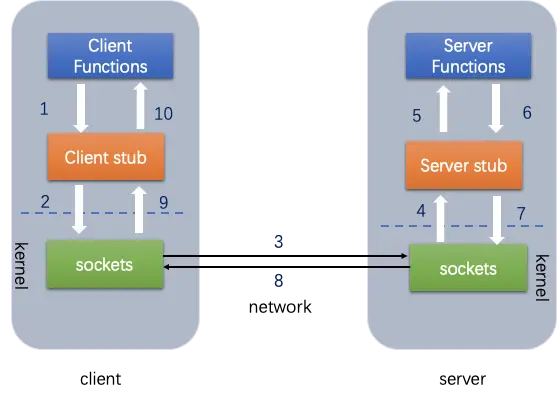
\includegraphics[width=.7\textwidth]{figures/RPC.svg}
    \caption{RPC流程图}
    \label{fig:rpc}
\end{figure}

图\ref{fig:rpc}展示了RPC调用流程。RPC通过桩(Stub)对应用屏蔽底层网络细节。客户端Stub将调用参数序列化,打包成网络消息发送给服务端;服务端的Stub将网络消息解包、反序列化得到调用参数,然后调用本地的服务程序;执行结束后,结果数据以类似的方式返回给客户的调用者。

\subsection{Rust语言}

Rust编程语言~\cite{rust-lang}是一种现代的系统级安全编程语言,其设计目标是在提供与C/C++类似的系统级编程能力的同时避免C/C++中常见的安全问题,例如缓冲区溢出、空指针引用等。Rust在编译阶段提供了强大的静态类型安全和内存安全保障,并成功将高级语言的功能性和表现力与无垃圾回收的运行时性能相结合。

Rust的所有权模型是其编译时内存安全和管理的关键。在Rust中,每个内存中的对象只能有且只有一个所有者,负责对象的初始化和析构;当这个对象被移动后,原来的所有者将无法再访问该对象。这种所有权模型可以避免内存泄漏和数据竞争等内存安全问题。Rust还提供了一种称为借用(borrowing)的内存安全的共享机制,类似于C++中的引用,但是有更严格的安全限制。Rust的所有权模型和借用机制可以在编译阶段检查出内存安全问题,而不需要运行时的垃圾回收机制。

Rust还有许多其他特性,例如生命周期分析、安全线程模型、零成本抽象、高级模块系统、Cargo管理工具等,这些特性使得Rust具备安全、高效、易用的特点,成为了开发高性能、安全可靠的系统级软件的理想选择。
